\documentclass[
	%a4paper, % Use A4 paper size
	letterpaper, % Use US letter paper size
]{jdf}

\addbibresource{references.bib}

\author{Nan Xiao}
\email{nanx@gatech.edu}
\title{CS6750 HCI Summer 2021:\\Assignment P5}

\begin{document}
%\lsstyle

\maketitle

\section{Question 1 - Computer Science Prompt}
\subsection{Positive effect of OMSCS}
The main reason for me and many others to choose OMSCS is its value. The program has a great reputation at an affordable cost. There are many low-cost online programs, but quality is also an important factor. From my point of view, the main positive effect of OMSCS is to make high-quality post-graduate education more accessible like never before. 

This positive effect comes in 2 ways. First, the low-cost structure enables those people who cannot afford normal university tuition to access post-graduate level education. Second, the flexible structure of the program enables full-time working adults to consider do a post-graduate degree in their free time.

\begin{figure}[h]
	\centering
	
\includegraphics[height=6cm]{jdf-latex/Figures/new_omscs_numbers.jpeg}
	\caption{Gatech OMSCS - Enable more people to access high quality postgraduate education}
	\label{fig:omscs}
\end{figure}

\subsection{Potential Negative effect of OMSCS}
Every coin has 2 sides. The low-cost structure makes the OMSCS program more accessible, but people tend to have a lower commitment as well. The drop-out rate of the OMSCS program is higher than the on-campus program, one of the reasons is that the sunk cost is much lower. People can afford to drop out with the minimum financial cost.
But there can be selection bias here as well. The low-cost structure enables much more people from lower-income families to participate in the program, but those people are much more likely to drop out because of the family issue. Also, another important factor for the high drop-out rate is that the OMSCS students are generally working adults with full-time jobs. There are much more life commitments comparing to the normal colleague students.

\begin{quotation}
\noindent "The demographics of OMSCS differ from MSCS: the average age of a starting OMSCS student is 32 as compared with 22 in MSCS, the majority of OMSCS students are domestic (67.1\% in Spring semester 2019), while MSCS' is international (55.4\%), most work a full-time job"
\end{quotation}

Many people dropped out from the OMSCS program because of the change of work and family commitment (e.g. Having a newborn to take care of).

\subsection{Design to preserve the positive effect and limit the negative effect}
To keep the program accessible at a low cost and encourage commitment and engagement, we can increase the cost of the program and give as much scholarship as possible to those who are in need. There can be performance-based awards as well. To encourage people with major life changes able to continue their education, we can allow people to pause the program for 6-12 months for a valid reason. 

\section{Question 2 - Computer Science Prompt}
\subsection{Area that political motivations are determining the design of technology}


Social media keeps people connected nowadays. There are many active designs and studies in this domain. The way people sharing and interacting with each other are heavily affected by political motivations. In China, the biggest social media is not Facebook or Instagram, it is the Moments within the super app WeChat. In this section, we will discuss the value-sensitive design of WeChat Moments and stakeholders with their motivations. The way WeChat Moments allows user to share their life and how they are interacting is very different from what you can do with Facebook or Instagram. 

\subsection{Stakeholders and their motivations}
We can refer to below Table 1 for the stakeholders and their motivations. There are clear conflicts between the users and the advertisers, the users want less annoying ads and the advertisers want the opposite. Tencent (WeChat company) would love to maximize the profitability but if user experience damages too much, they could lose users to competitors. And the company can be in trouble with regulators if they misuse the user data. So they have to carefully design the product that according to the Chinese culture's value and minimize the negative impact by monetization.

\begin{table}[h] % [h] forces the table to be output where it is defined in the code (it suppresses floating)
	\caption{WeChat Moments - Stakeholders and their motivations}
	\small % Reduce font size
	\centering % Centre the table
	\begin{tabular}{L{0.2\linewidth} L{0.7\linewidth} }
		\textbf{Stakeholders} & \textbf{Motivations} \\
		\toprule[0.5pt]
		WeChat Company & High user engagement, high user activities to make ads slots more valuable, profitability \\
		\midrule
		WeChat Users & User privacy is concerned, free to post without judgement, interaction with friends, less ads \\
		\midrule
		Advertisers & High user activities, more people to see their ads \\
		\midrule
		Regulators & User data is protected, users are free from social media scams \\
		\midrule
		Competitors & Focus on the bad experience part of WeChat Moments and offer a better product \\
	\end{tabular}
\end{table}

\subsection{Motivations affecting the design of the technology}
\begin{figure}[h]
	\centering
	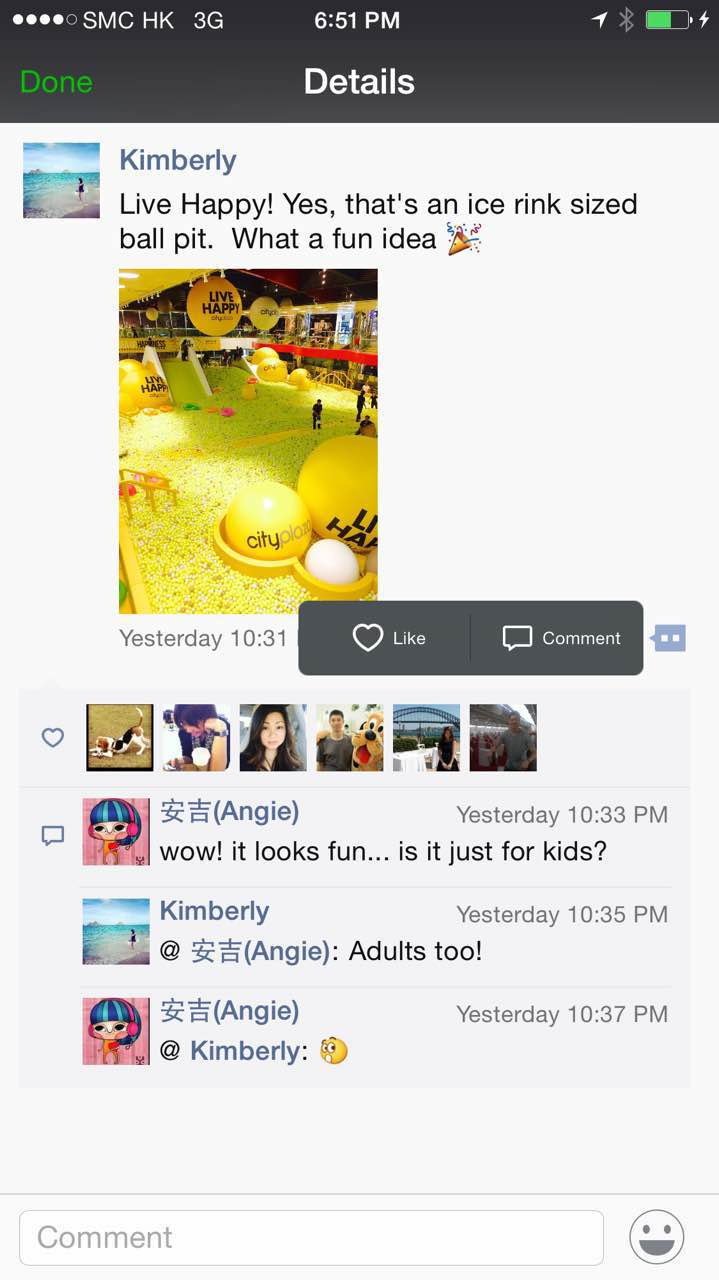
\includegraphics[height=6cm]{jdf-latex/Figures/wechat.jpg}
	\caption{WeChat Moments - Value sensitive design}
	\label{fig:wechat}
\end{figure}

From Figure 1 we can see a particular post of WeChat Moments. The core value of the WeChat design is to take care of user privacy. It is very different from another social media platform called Weibo, which is like Twitter. Everyone can see others' posts. The post can only be seen by the friends added. Also, you can set up group view access to allow only a small portion of people to see your posts. Through this design, WeChat emphasizes the privacy of the users and let them choose who can see their posts. This is tailored to WeChat's motivation, because they want to have more user engagements, and encourage users to do more posting. The ultimate goal is to boost the engagement that they can sell other services like WeChat pay, and more advertising on the platform. The design concerns about privacy also lower the barriers for users to do posting, they can share some sensitive posts with close friends only.


\section{Question 3 - ACM CHI}

\subsection{Paper 1}
(\cite{10.1145/3313831.3376442})
\subsubsection{Title and Author}
Paper Title:
\begin{quotation}
\noindent "Wrex: A Unified Programming-by-Example Interaction for Synthesizing Readable Code for Data Scientists" 
\end{quotation}

Authors:
\begin{quotation}
\noindent "Ian Drosos, Titus Barik, Philip J. Guo1, Robert DeLine, Sumit Gulwani"
\end{quotation}

\subsubsection{Summary}
This paper proposes a new programming-by-example way for the data scientist to do data wrangling. Traditionally, data scientist has a variety of data wrangling tools to use, but they are reluctant to do so. Because to use those tools requires data scientists to leave their programming environment - Jupyter notebook, and often in another programming language than Python. The authors present a new tool embedded in the Jupyter notebook using the same python language, which will make it easier for data scientists to adopt the new tool to the workflows.

\begin{figure}[h]
	\centering
	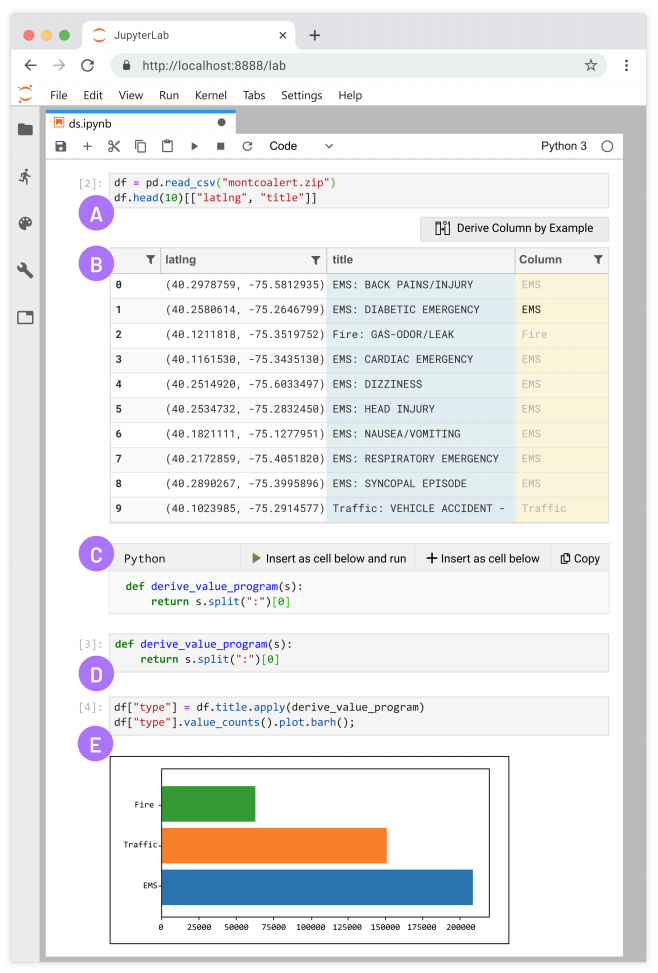
\includegraphics[height=6cm]{jdf-latex/Figures/wrex.png}
	\caption{WREX - Jupyter notebook extension to do data wrangling}
	\label{fig:wrex}
\end{figure}

\subsubsection{Interesting point}
First, as a 6 years data scientist, I agree with the author that the data wrangling tools are generally ignored by professional data scientists. We normally have to write code with libraries like Numpy, Pandas and Matplotlib to understand how to do the proper data wrangling. But if there is a widget in the jupyter notebook to speed up this process, it is going to be helpful. The authors used the familiar interface to bridge the gulf of execution for the end-users. 

Second, the authors have done enough research on the need-findings. There are many tasks for a data scientist to deliver a data product. Data wrangling is the most time consuming one but less interesting. This is a great area to design a product for improving workflow efficiency. The authors also did both qualitative research and quantitative research to make sure the tool is indeed improving the data scientist's efficiency.


\subsection{Paper 2}
(\cite{10.1145/3313831.3376131})
\subsubsection{Title and Author}
Paper Title:
\begin{quotation}
\noindent "If I Hear You Correctly: Building and Evaluating Interview Chatbots with Active Listening Skills" 
\end{quotation}

Authors:
\begin{quotation}
\noindent "Ziang Xiao, Michelle X. Zhou, Wenxi Chen, Huahai Yang, Changyan Chi"
\end{quotation}

\subsubsection{Summary}
This paper is written by a joint effort of UIUC and Juji.\footnote{Here is the websites of \href{https://dais.cs.illinois.edu/}{UIUC DAIS}, and \href{https://juji.io/}{Juji, Inc}, ACM SIGCHI paper \href{https://dl.acm.org/doi/abs/10.1145/3313831.3376131}{link}.} It proposed an active-listening chatbot for the interview process. The current chatbot is usually not good at handling free context out of its training domain. Especially for interview chatbot, it is more functioning as a better way to do form filling. But by leveraging the latest progress in natural language processing and chatbot technology, Juji can build a chatbot to handle users' free-text responses and open-ended questions. This is great progress to enhance the user experience when they are interacting with a chatbot.

\begin{figure}[h]
	\centering
	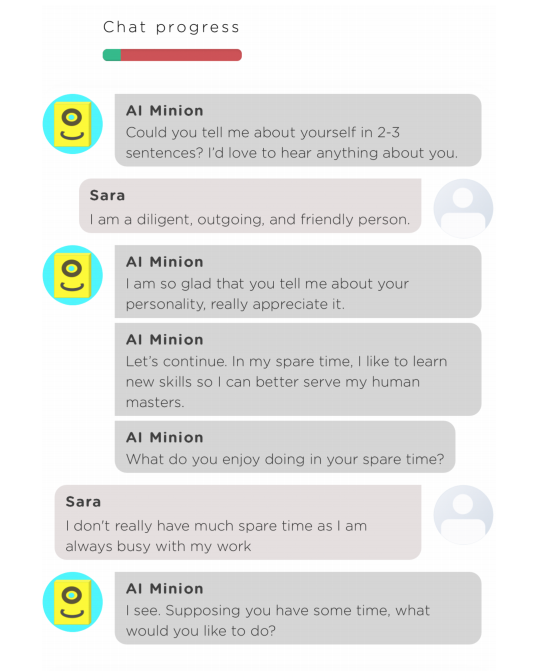
\includegraphics[height=6cm]{jdf-latex/Figures/chatbot.png}
	\caption{A screenshot of an example interview conducted
by a chatbot (AI Minion) and a user (Sara).}
	\label{fig:chatbot}
\end{figure}



\subsubsection{Interesting point}
The current chatbot technology is usually context-based, for example, identify if you are interested in booking a flight or hotel, or request for particular service, then redirect you to the preset workflows. The chatbot will fill the slot by asking standard questions like, what is your check-in date, your destination, your account number, etc. They cannot handle out-of-context questions or responses. Some chatbots and do casual chatting if your first question is labelled as small-chat for example. But once you are in the flow, the chatbot is poor at handling free-text responses. The new chatbot Juji proposed can handle that during the user conversation and that makes the users feel more like talking to a real agent than a robot. The new design fits more to the predictor model of the user. The user would expect a natural response when giving a free-text response or asking open-ended questions.

\section{Question 4 - Other Conferences}

\subsection{Conference 1 - International Conference on Human-Robot Interaction}
This is one of the best full paper awards of the International Conference on Human-Robot Interaction 2021 on Technical Advances Track. \footnote{Awards HRI 2021 \href{https://humanrobotinteraction.org/2021/awards/}{link}} And it is from Georgia Tech RAIL Lab.
(\cite{10.1145/3434073.3444657})
\subsubsection{Title and Author}
Paper Title:
\begin{quotation}
\noindent "Explainable AI for Robot Failures: Generating Explanations that Improve User Assistance in Fault Recovery" 
\end{quotation}

Authors:
\begin{quotation}
\noindent "Devleena Das, Siddhartha Banerjee, Sonia Chernova"
\end{quotation}

\subsubsection{Summary}
In this paper, the author proposed a new way of interpreting error messages using explainable for novice users. The author proposed a new type of explanation, Eerr, to help the non-expert users understand robot failure and identify solutions. By using the explainable AI approach, they can generate meaningful explanations for unseen scenarios as well. This is very helpful for the non-expert users to understand the problems of the robot and act accordingly to fix the issue.


\subsubsection{Interesting point}
The authors have creatively adopted the explainable AI methods to robot failures. It is one of the hottest areas in the machine learning field and it make sense to adopt some best practices in the robotic field. Especially, the failures of a robot are almost inevitable during the development phase and moving from the testing environment to the real world. 

\subsection{Conference 2 - International Conference on Tangible, Embedded, and Embodied Interaction}
This is the best paper award of International Conference on Tangible, Embedded, and Embodied Interaction 2020. \footnote{Awards TEI 2020 \href{https://tei.acm.org/2020/}{link}}
(\cite{10.1145/3374920.3374924})
\subsubsection{Title and Author}
Paper Title:
\begin{quotation}
\noindent "ForceStamps: Fiducial Markers for Pressure-sensitive Touch Surfaces to Support Rapid Prototyping of Physical Control Interfaces" 
\end{quotation}

Authors:
\begin{quotation}
\noindent "Changyo Han, Katsufumi Matsui, Takeshi Naemura"
\end{quotation}
\subsubsection{Summary}
The authors proposed ForceStamps, fducial markers for supporting the rapid prototyping of physical control interfaces on pressure-sensitive touch surfaces. The authors also showcased a wide range of physical controls could be prototyped by utilizing the characteristics of the buffer materials and the spatial constraints.

\subsubsection{Interesting point}
We rarely understand how to design and rapid prototyping for the haptic sense. It is an interesting and useful design that enable designers without knowledge of electronics to be able to design for touch interface. ForceStamps bridges the gulfs of execution and gulfs of evaluation between the user and the design task. Also, from the example, we can see that it allows the designer to directly manipulate through the interface. This interface further shortens the path between the user and the task.

\begin{figure}[h]
	\centering
	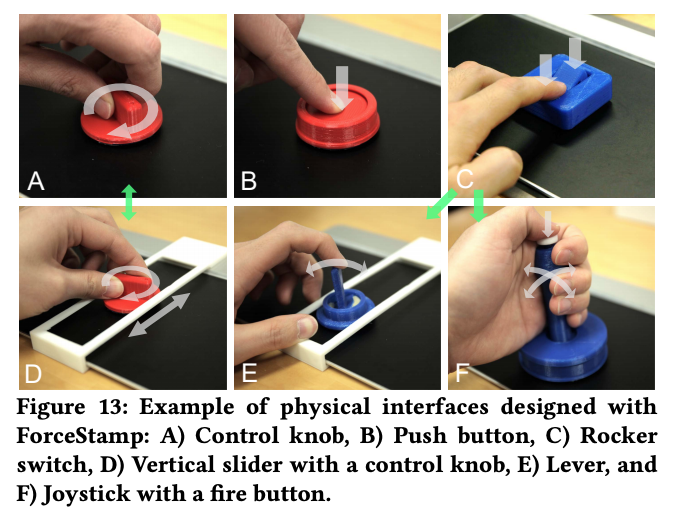
\includegraphics[height=6cm]{jdf-latex/Figures/ForceStamps.png}
	\caption{ForceStamps - Direct Manipulation}
	\label{fig:forcestamp}
\end{figure}

\section{References}
\printbibliography[heading=none]

\end{document}